%package list
\documentclass{article}
\usepackage[top=3cm, bottom=3cm, outer=2cm, inner=2cm]{geometry}
\usepackage{graphicx}
\usepackage{hyperref}
\usepackage{array}
\newcolumntype{x}[1]{>{\centering\arraybackslash\hspace{0pt}}p{#1}}
\usepackage[english,spanish]{babel}
\usepackage[utf8]{inputenc}
\usepackage{fancyhdr}
\usepackage{enumitem}
\usepackage{tikz-qtree}
\usepackage{tikz}
\usetikzlibrary{arrows.meta,bending}
\tikzset{every tree node/.style={minimum width=2.5em,draw,circle},
     blank/.style={draw=none},
     edge from parent/.style=
     {draw, edge from parent path={(\tikzparentnode) -- (\tikzchildnode)}},
     level distance=1.5cm}
\usepackage{minted}
\usetikzlibrary{shapes}

%%%%%%%%%%%%%%%%%%%%%%%%%%%%%%%%%%%%%%%%%%%%%%%%%%%%%%%%%%%%%%%%%%%%%%%%%%%%
\newcommand{\csemail}{vmachacaa@unsa.edu.pe}
\newcommand{\csdocente}{Vicente Machaca Arceda}
\newcommand{\cscurso}{Algoritmos y Estructura de Datos}
\newcommand{\csuniversidad}{Universidad Nacional de San Agustín}
\newcommand{\csescuela}{Maestría en Ciencia de la Computación}
\newcommand{\cspracnr}{Final}
\newcommand{\cstema}{Trabajo final}
%%%%%%%%%%%%%%%%%%%%%%%%%%%%%%%%%%%%%%%%%%%%%%%%%%%%%%%%%%%%%%%%%%%%%%%%%%%%


\AtBeginDocument{\selectlanguage{spanish}}
\renewcommand{\figurename}{Figura}
\renewcommand{\refname}{Referencias}
\renewcommand{\tablename}{Tabla}
\AtBeginDocument{
	\renewcommand\tablename{Tabla}
}

\pagestyle{fancy}
\fancyhf{}
\setlength{\headheight}{30pt}
\renewcommand{\headrulewidth}{1pt}
\renewcommand{\footrulewidth}{1pt}
\fancyhead[L]{\raisebox{-0.2\height}{
\includegraphics[width=3cm]{img/logo_unsa}}}
\fancyhead[C]{}
\fancyhead[R]{\fontsize{7}{7}\selectfont	\csuniversidad \\ \csescuela \\ \textbf{\cscurso} }
\fancyfoot[L]{MSc. Vicente Machaca}
\fancyfoot[C]{\cscurso}
\fancyfoot[R]{Página \thepage}

\usemintedstyle{vs}

\begin{document}
	\vspace*{10px}
	
	\begin{center}	
		\fontsize{17}{17} \textbf{ Práctica \cspracnr}
	\end{center}

	\begin{table}[h]
		\begin{tabular}{|x{5.4cm}|x{5.4cm}|x{5.4cm}|}
			\hline 
			\textbf{DOCENTE} & \textbf{CARRERA}  & \textbf{CURSO}   \\
			\hline 
			\csdocente & \csescuela & \cscurso    \\
			\hline 
		\end{tabular}
	\end{table}	
	
	\begin{table}[h]
		\begin{tabular}{|x{5.4cm}|x{5.4cm}|x{5.4cm}|}
			\hline 
			\textbf{PRÁCTICA} & \textbf{TEMA}  & \textbf{DURACIÓN}   \\
			\hline 
			\cspracnr & \cstema & 3 horas   \\
			\hline 
		\end{tabular}
	\end{table}
	
	\section{Datos de los estudiantes}
	\begin{enumerate}
		\item \textbf{Grupo:} 09
		\item \textbf{Integrantes:}
		\begin{itemize}
			\item Asmat Fuentes, Franz Rogger
			\item Esthela Espinoza, Fausto Danilo
			\item Ojeda Mamani, Abel Eberth
			\item Paredes Rodriguez, Raybert
		\end{itemize}		
	\end{enumerate}
	
	\section{Implementación KD Tree}\label{sec:trabajo}
	\begin{enumerate}
        
        \item \textbf{Introducción:}  El presente trabajo pretende hacer una implementación del algoritmo KDTree y la búsqueda K-Nearest Neighbor (KNN), explora el concepto de usar una estructura de datos de árbol KD para identificar los colores cercanos en base a una selección de una paleta de colores dada.

        El código fuente de esta disponible en: 
        
        \begin{center}
	        \url{https://github.com/UNSA-MCC-2022/AyED_Trabajo_Final}
	    \end{center}

        Se pretende establecer una búsqueda de colores cercanos a uno seleccionado por el usaurio, retornando el nombre de esos colores cercanos en base a una paleta pre-establecida. En lugar de adivinar un color al azar, estamos tratando de limitar nuestras conjeturas a una lista seleccionada de colores. Un escenario de ejemplo sería analizar las fotos de productos de un catálogo de productos conocido con colores estándar.
        
        Se ha construido una paleta de colores en datos (JSON), en base a ello se realizarán las búsquedas, con este conjunto de datos se pretende realizar las búsquedas utilizando KNN, a continuación se muestra una porción de esta información:
        
        \begin{center}
            \frame{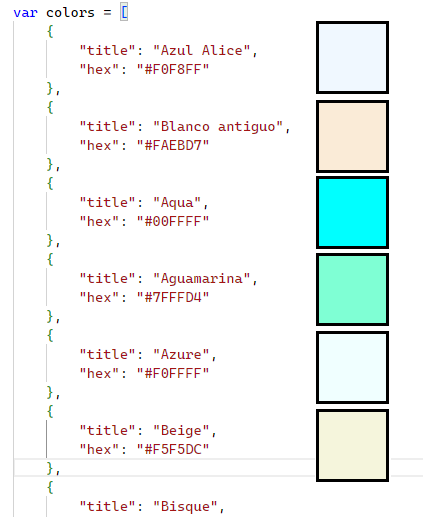
\includegraphics[width=10cm]{img/paleta}}\par
            \textit{Figura 1: Paleta de colores en datos}
        \end{center}
        
        \item \textbf{Utilización:}  Para el píxel del color seleccionado, elegiremos los color más similares de la paleta anterior. Básicamente, necesitamos convertir la el color en sus componentes RGB para que todos los colores resultado de la búsqueda sean de la paleta.

        Para ello, se necesita definir qué es la similitud de color. El enfoque más sencillo sería considerar el hecho de que cada color se compone de tres componentes: rojo, azul y verde, como un punto tridimensional. Si los representamos en un gráfico con valores de rojo, verde y azul como los tres ejes, podemos ver que los similares permanecen cerca uno del otro:

        \begin{center}
            \frame{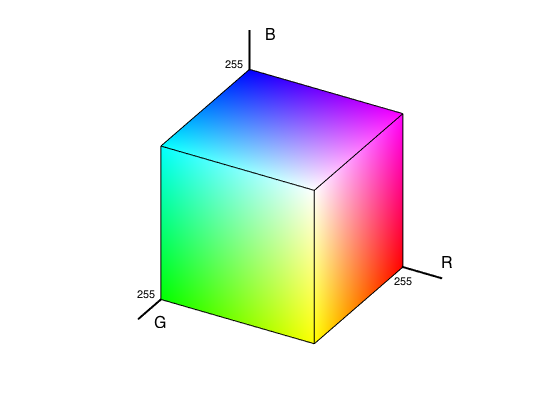
\includegraphics[width=10cm]{img/rgb_3d}}\par
            \textit{Figura 2: Representación 3D de los componentes RGB}
        \end{center}

        Una vez definida la forma de descomponer el color en partes, lo siguiente es conocer que para encontar los colores similares, estos tienen los componentes RGB cercanos entre si. Es en ese pounto en que entra KNN, con este algorimo podemos encontrar puntos 3D cercanos entre si.
        
        Para realizar esto se debe calcular la distancia entre los diferentes colores. En un sistema de coordenadas cartesianas 3D como el de la imagen, la ecuación de la distancia entre dos colores sería:

        \[\sqrt{(r_1 - r_2)^2 + (g_1 - g_2)^2 + (b_1 - b_2)^2}\]

        Donde:
        \[(r_1, \; g_1 \; y \; b_1)\]
        \begin{center}
            \textit{ Son del primer color y }
        \end{center}
        \[(r_2, \; g_2 \; y \; b_2)\]
        \begin{center}
            \textit{ del segundo color }
        \end{center}

        Podemos encontrar la distancia entre el color de cada píxel contra cada uno de los colores de la paleta y encontrar el color de la paleta más similar.

        \item \textbf{Implementación:} Para realizar las acciones anteriormente mencionadas se procede mostramos la implementación de KNN (en la función nearest del archivo kdtree.js)

            \begin{minted}
            [
                frame = lines,
                framesep = 2mm,
                obeytabs = true,
                tabsize = 2
            ]
            {javascript} 
        // Algoritmo K-Nearest Neighbor(KNN)
        function nearest (point, maxNodes, maxDistance) {
        	var i,
        		result,
        		bestNodes;
        
        	bestNodes = new BinaryHeap(
        		function (e) { return -e[1]; }
        	);
        
        	function nearestSearch(node) {
        		var bestChild,
        			dimension = dimensions[node.dimension],
        			ownDistance = metric(point, node.obj),
        			linearPoint = {},
        			linearDistance,
        			otherChild,
        			i;
        
        		function saveNode(node, distance) {
        			bestNodes.push([node, distance]);
        			if (bestNodes.size() > maxNodes) {
        				bestNodes.pop();
        			}
        		}
        
        		for (i = 0; i < dimensions.length; i += 1) {
        			if (i === node.dimension) {
        				linearPoint[dimensions[i]] = point[dimensions[i]];
        			} else {
        				linearPoint[dimensions[i]] = node.obj[dimensions[i]];
        			}
        		}
        
        		linearDistance = metric(linearPoint, node.obj);
        
        		if (node.right === null && node.left === null) {
        			if (bestNodes.size() < maxNodes || ownDistance < bestNodes.peek()[1]) {
        				saveNode(node, ownDistance);
        			}
        			return;
        		}
        
        		if (node.right === null) {
        			bestChild = node.left;
        		} else if (node.left === null) {
        			bestChild = node.right;
        		} else {
        			if (point[dimension] < node.obj[dimension]) {
        				bestChild = node.left;
        			} else {
        				bestChild = node.right;
        			}
        		}
        
        		nearestSearch(bestChild);
        
        		if (bestNodes.size() < maxNodes || ownDistance < bestNodes.peek()[1]) {
        			saveNode(node, ownDistance);
        		}
        
        		if (bestNodes.size() < maxNodes || Math.abs(linearDistance) < bestNodes.peek()[1]) {
        			if (bestChild === node.left) {
        				otherChild = node.right;
        			} else {
        				otherChild = node.left;
        			}
        			if (otherChild !== null) {
        				nearestSearch(otherChild);
        			}
        		}
        	}
        
        	if (maxDistance) {
        		for (i = 0; i < maxNodes; i += 1) {
        			bestNodes.push([null, maxDistance]);
        		}
        	}
        
        	if (self.root)
        		nearestSearch(self.root);
        
        	result = [];
        
        	for (i = 0; i < Math.min(maxNodes, bestNodes.content.length); i += 1) {
        		if (bestNodes.content[i][0]) {
        			result.push([bestNodes.content[i][0].obj, bestNodes.content[i][1]]);
        		}
        	}
        	return result;
        }
        \end{minted}            
  
    \item \textbf{Prueba en browser:} A continuación s epresenta la ejecución del codigo en browser, en el ejempo se puede apreciar que al elegir un color en el selector de colores, se muestran los diez (10) coolores mas cercanos a la paleta de colores predefinida.

    \begin{center}
        \frame{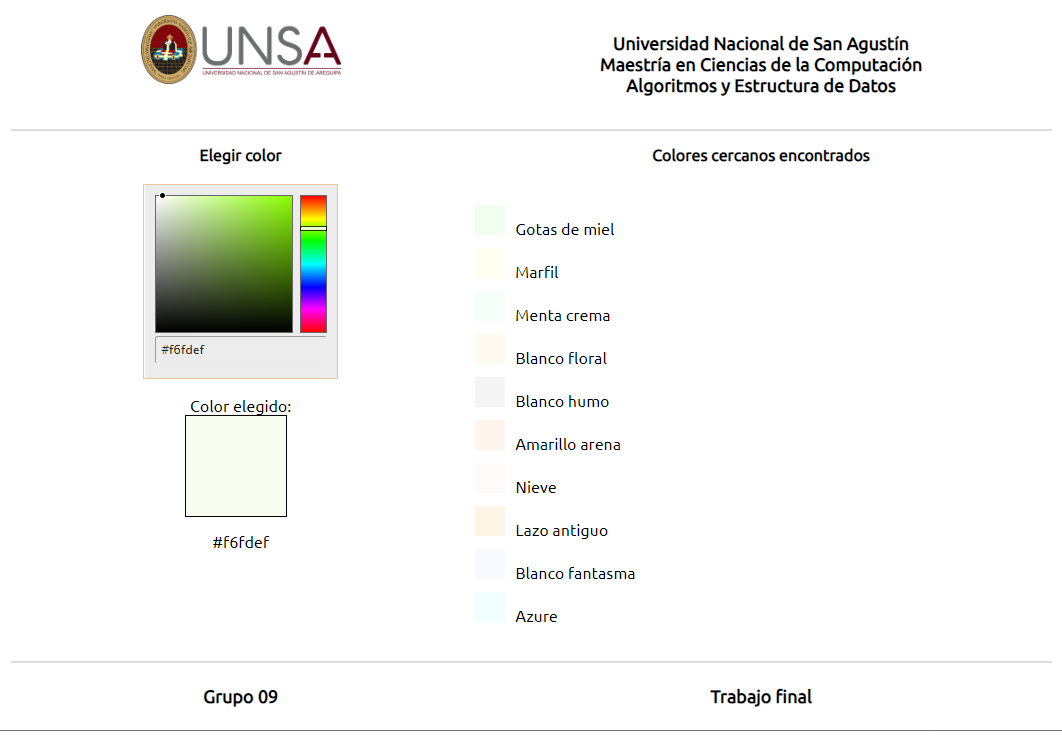
\includegraphics[width=15cm]{img/ejecucion}}\par
        \textit{Figura 3: Busqueda de colores en ejecucion}
    \end{center}
  
    \item \textbf{Conclusiones:}  El método del árbol kd En pocas palabras, se crea una estructura de datos en forma de árbol para almacenar la paleta base. Esto preservará la información sobre la cercanía de cada color entre sí en la propia estructura de datos. Cuando se busca un color similar, en lugar de calcular la distancia a todos los colores de la paleta y se calculam solo a los pocos más cercanos, ahorrando el cálculo.

    En base a lo realizado, el metodo indicado puede ser usado para reconocimiento de colores dentro de imágenes convirtiendo la imagen en pixeles tratando de ubicar elementos dentro de la imagen, como por ejemplo:

    \begin{center}
        \frame{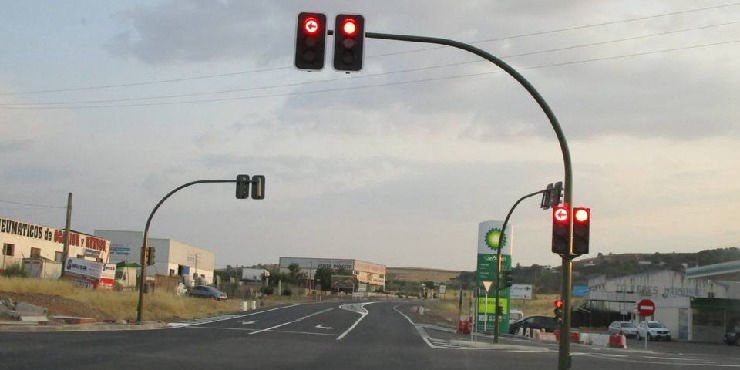
\includegraphics[width=12cm]{img/semaforo}}\par
        \textit{Figura 4: Semaforo}
    \end{center}

    Una vez obtenida una paleta cercana a las imagenes que se queiren analizar, el siguiente paso sería agrupar los colores cercanos a cuando el semaforo esta encendido o apagado en cierta luz, 

    \begin{center}
        \frame{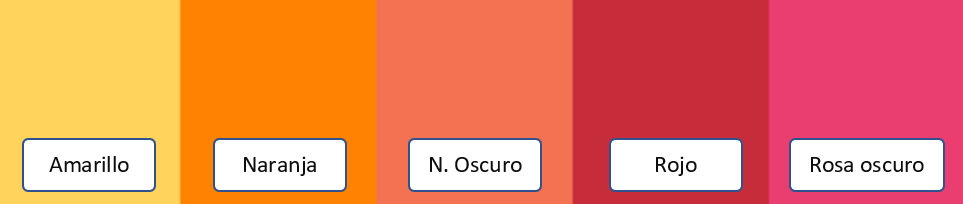
\includegraphics[width=10cm]{img/colores}}\par
        \textit{Figura 5: Paleta de color cercano al semaforo}
    \end{center}

    Con los colores cercanos y agrupados hasta obtener cierta cereza que la luz del semaforo esta encendida o apagada


    \end{enumerate}
    
    \section{Repositorio}\label{sec:codigo}
        La implementación de los algoritmos y los datos utilizados es el siguiente:\par
	    \par
	    \begin{center}
	        \url{https://github.com/UNSA-MCC-2022/AyED_Trabajo_Final}
	    \end{center}

    \section{Representación gráfica}\label{sec:representacion}
        Se realizó la implementación de la representación gráfica de los algoritmos indicados, esto se pueden visualizar en el siguiente enlace:\par
	    \par
	    \begin{center}
	        \url{https://unsa-mcc-2022.github.io/AyED_Trabajo_Final/docs/index.html}
	    \end{center}

\end{document}